
\section{Statistical Modelling Basics}

Statistical modelling is the process of constructing mathematical models for data that arise from random processes. Statistical inference involves using these models to infer things about the generating processes. 

%Figure 9 illustrates this. Statistical modelling is required whenever we want to understand how data, ${\bf y}$ are generated by a stochastic process (i.e. a process involving randomness). It involves proposing a statistical model to explain how the data are generated, i.e. how the data arise from the parameters $\bm{\gamma}$ of the process that we know, the explanatory variables ${\bf x}$ that we know, and possibly some parameters $\bm{\theta}$ that we don't know. If there are some parameters that we don't know and are interested in knowing, we can use the statistical model together with observed the data ${\bf y}$, to infer the values of the parameters that we don't know. This process is called statistical inference, and is the focus of most of the rest of this module.

%\begin{figure}[ht!]
%\caption{\small Schematic representation of statistical modelling. We propose a statistical model (a pdf or pmf) to explain how the data $y$ are generated, i.e. how the data arise from the parameters $\bm{\gamma}$  that we know, the explanatory variables $\bm{x}$ that we know, and the parameters $\bm{\theta}$ that we don't know. Then once we observe the data, we use this statistical model (in the form of a likelihood function) to infer the values of the parameters that we don't know.}
%\centering
%\includegraphics[width=0.9\textwidth]{StatmodFigure.pdf}
%\label{fig:StatmodFigure}
%\end{figure}

There are a number of ways of doing statistical inference. The two main ones go under the names of ``frequentist inference" (also called ``classical inference'') and ``Bayesian inference". %Here we focus mainly on the former, but if you aspire to do applied statistics you really need to be familiar with both methods of inference. \todo[inline]{David says: Chris, this stuff is from a module I developed on maximum likelihood infrence - maybe we should add some basic Bayesian stuff to this document to make it more general?}

Both Bayesian and frequentist methods are based on likelihood functions. So proposing an appropriate likelihood function is absolutely central to developing a statistical model and to doing statistical inference. It is what links the things we observe (which include some random deviations from what is expected) to the things that we want to find out about but can't observe. It is different from the kinds of equations you will have dealt with in maths courses in that it includes a mathematical expression of the \textit{randomness} in the process.

The likelihood function is a quantitative description of the process that (we postulate) generated the observed data. The first step in statistical inference is identifying or proposing a probability distribution (which specifies the form of the randomness in the process) that might plausibly have generated the data.


\subsection{Likelihood functions}

A likelihood function is an expression that quantifies the likelihood of getting the observations you got. It is just a probability distribution function (PDF - if your data are continuous) or probability mass function (PMF - if your data are discrete). It contains some unknown parameters $\bm{\theta}$ (the things you want to estimate). For the purposes of inference, we treat the data as known values (after you observe them, they are known) and the parameters $\bm{\theta}$ as the things that the likelihood function depends on (they are unknown). Before you observe data, you have an expression that tells you the probability of getting any particular dataset. After you observe the data, you can use this to evaluate how likely any particular parameter values ($\bm{\theta}$) were to have generated the dataset.

Formulating likelihoods is just a question of writing down a PMF or PDF for the data you observed. This can be harder than it sounds. (For brevity, we will use the term ``probability distribution'' or just ``distribution'' to refert to PMFs and PDFs.)

\subsection{Building blocks: probability distributions}

The first step in obtaining a suitable likelihood is identifying a suitable PDF or PMF for the data at hand, and a first step in doing this is asking yourself whether the response (the random variable you are modelling - typically on the $y$-axis of a plot) is a continuous random variable (can take on values on a real line, e.g. anything between $-\infty$ and $\infty$, or between $0$ and $\infty$, or between $0$ and $1$), or a discrete random variable (can take on only specific discrete values, e.g. integers, or non-negative integers, or only the value $0$ or the value $1$). If it is continuous, you want to consider only PDFs; if it is discrete, you want to consider only PMFs.

Figure~\ref{fig:distributions} shows some common distributions, together with some of the relationships between them. In this figure, $n$ indicates counts (a discrete random variable), $\delta$ is a binary (and so discrete) random variable (0 or 1) and other responses are continuous. Among the continuous random variables, $t$ represents waiting time when on the left of ``$\sim$''and the $t$-distribution when on the right of it. 

The Poisson distribution is the ``mirror image'' of the exponential in the sense that if events occur randomly at an average rate of $\lambda$ then the waiting time between events has an exponential distribution with parameter $\lambda$, while the number of events occurring in an interval of length 1 has a Poisson distribution with parameter $\lambda$ (and the number of events occurring in an interval of length $t$ has a Poisson distribution with parameter $\lambda t$). The exponential's currency is time-per-event, while the Poisson's currency is events-per-time.\\

\begin{figure}[ht!]
\caption{\small Some common probability density and probability mass functions and some of the relationships between them.}
\centering
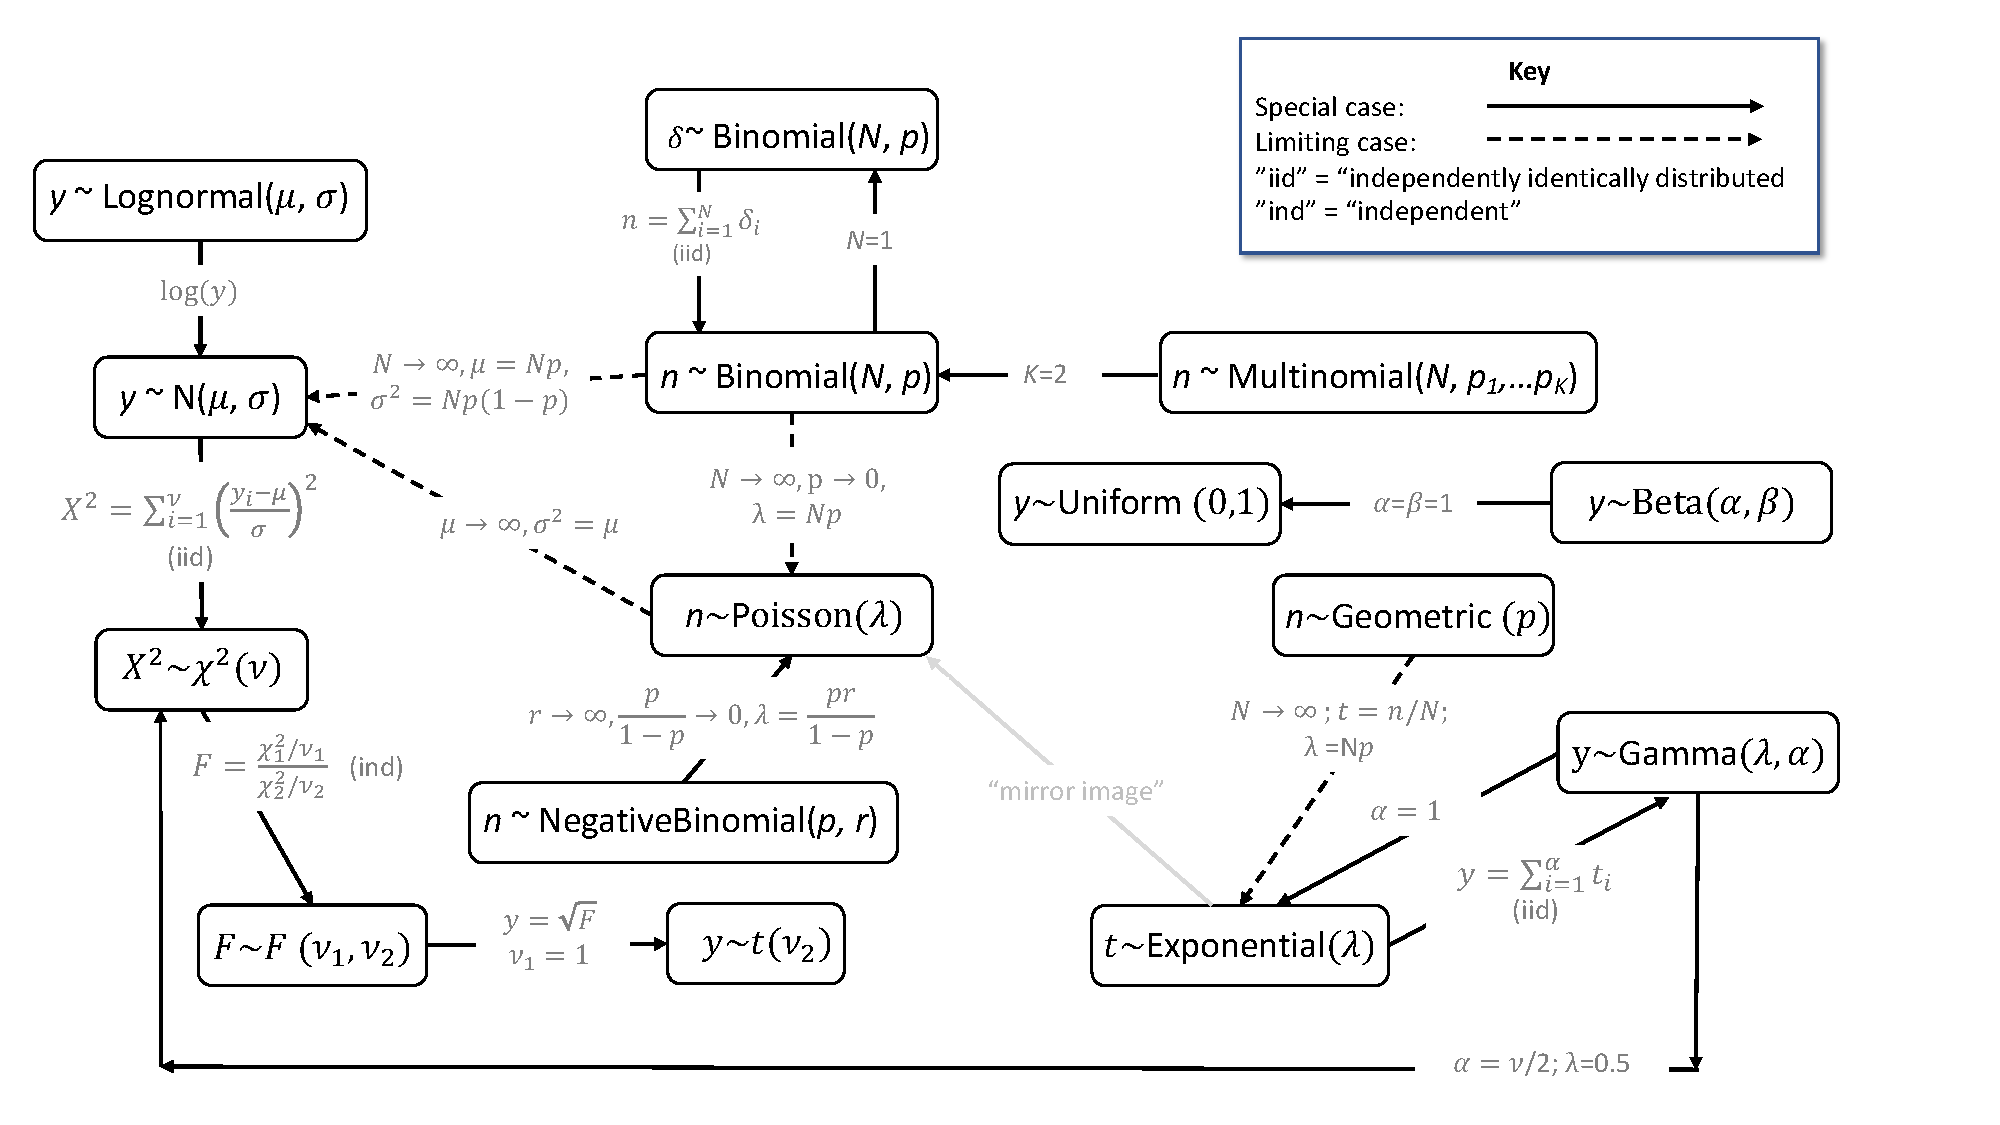
\includegraphics[width=1.1\textwidth]{distributions.pdf}
\label{fig:distributions}
\end{figure}


\begin{table}[ht]
\caption{Rough guide as to what each of the distributions in Figure~\ref{fig:distributions} is used for. The distributions in the top section of the table are PMFs for discrete random variables, while those in the bottom section are PDFs for continuous random variables.
\label{tab:distributions}}
\begin{center}
\begin{tabular}{rl}
\hline
PDF or PMF & Typical Use\\
\hline
Bernoulli & Used for binary data (e.g. success/failure, Yes/No).
\\
Binomial & Used for count data when there are a fixed number ($N$) of ``trials'', a \\
         & binary outcome for each trial, and the count is the number of ``successes''.
\\
Multinomial & Used for count data when there are a fixed number ($N$) of ``trials'' and \\
            & more than two possible kinds of outcome for each trial\\
Poisson & Used for count data when there is no limit on the size of the count, e.g. when \\
        & events occur at some  rate and we count the number of events in some interval.
\\
Negative Bionomial & Used as alternative to the Poisson distribution, when the variance \\
        & may be larger than the mean. 
\\
Geometric & Used for counts of number of events until the first ``success'', i.e. number of \\
          & events until some particular thing (a ``success'') occurs.
\\
\hline
Uniform & Used when all values in some interval are equally likely. \\
Exponential & Used for waiting time until some event. Similar to Geometric, but with \\
            & continuous wait time, instead of integer number of events. 
\\
Gamma & Generalisation of the Exponential to allow greater or lesser variance.
\\
Beta & Used for modelling the distribution of probabilities or proportions \\
     & (numbers between 0 and 1). \\
Normal & Used to model continuous random variables that can have values anywhere \\
       & on the real line (positive or negative). Use often justified by the Central \\
       & Limit Theorem.
\\
Lognormal & Used to model continuous random variables that can have values anywhere \\
       & on the real line greater than or equal to zero.
\\
$\chi^2$ & Used for squared standardised normal random variables.
\\
$F$ & Used for ratio of two independent Chi-squared random variables.
\\
$t$ & Special case of the F distribution; used for continuous random variables with \\
  & heavier tails than the Normal distribution.
\\
\hline
\end{tabular}
\end{center}
\label{default}
\end{table}

\clearpage

Consider Figure~\ref{fig:distributions} and Table~\ref{tab:distributions} to be the building blocks for likelihood functions. The first step in building an appropriate likelihood function for your data is identifying which of these blocks it is made out of.

\subsection{Suggest an appropriate distribution}

Here's an exercise in suggesting distributions appropriate for different kinds of data. For each of the scenarios below, propose at least one appropriate distribution.

\begin{enumerate}

\item A survey in which you count the number of daisies in randomly-chosen 1m$^2$ quadrats in a field.

\item A survey in which you count the number of females in a sample of $N$ animals.

\item A survey in which you are told only the proportion (not the numbers) of males in the catches of 10 fishing boats.

\item A survey in which you count the numbers of fish in each of 6 age classes in a catch of 100 fish.

\item A survey in which you record which of 100 ringed birds returns to its breeding site the following year.

\item A survey in which you count the number of attempts it takes a squirrel to get from the ground to a bird feeder hung high in a tree.

\item A survey in which you time how long it takes the squirrel to get to the bird feeder.

\item A survey in which you count the number of individuals that are photographed by a camera trap in a week.

\item A survey in which you observe the times between animals being photographed by a camera trap.

\item A survey in which you observe the weights of 50 praying mantis.

\item A survey in which you observe the mean weights of catches landed by 50 fishing boats.

\end{enumerate}
\subsection{Some useful facts about some distributions}

\textit{Hot tip: Wikipedia is an excellent source of information about probability distributions.}

\begin{enumerate}

\item \textbf{Mean-variance relationships} 

The relationship between the mean and the variance of many common probability distributions is ``hard-wired''. Some examples:

  \begin{enumerate}
  \item The mean of a Poisson distribution with parameter $\lambda$, is $\lambda$, and so is its variance.
%  \item The mean of a binomial distribution with parameters $N$ and $p$, is $Np$, and its variance is $Np(1-p)$.
  \item The mean of an exponential distribution with parameter $\lambda$, is $1/\lambda$, and its variance is $1/\lambda^2$.
  \item The mean of a geometric distribution with parameter $p$, is $1/p$, and its variance is $(1-p)/p^2$.
  \end{enumerate}
  
The normal distribution, with which most people are most familiar, is somewhat unusual in that its variance does not depend on its mean at all. This gives it additional flexibility. 

The gamma distribution is used to give the exponential distribution this kind of additional flexibility; by adding another parameter ($\alpha$) we get the flexibility to have the variance not depend on the mean.

In a similar way, the negative binomial distribution allows the variance of count random variables to be greater than the mean (unlike the case with Poisson counts), having an extra parameter ($r$) that controls the distribution's variance.

\item \textbf{``Thinned'' Poisson distribution}

Suppose that the number of things (e.g. animals in a population) is a Poisson random variable with parameter $\lambda$, and each of these things is detected independently with the same probability, $p$, then the number of \textit{detected} things is also a Poisson random variable, but with parameter $\lambda p$. The number of things is said to have been ``thinned'' by the detection probability $p$.

The Poisson distribution is unusual in this respect. It is generally the case that if the number of animals in a region has some given probability distribution, then the number of \textit{detected} animals will have an entirely different kind of distribution. But if the number of animals in a region has a Poisson distribution, then the number of \textit{detected} animals also has a Poisson distribution. This is a very convenient feature of the Poisson distribution.

\item \textbf{Poisson-Multinomial relationship}

Suppose the number of each of $K$ kinds of things is a Poisson random variable, with the $k$th kind having parameter $\lambda_k$, then if we ``condition on'' the total number of things, $N$, that were generated by these Poisson distributions (``conditioning on $N$'' means here ``once we know $N$''), then the number of things of each kind has a multinomial distribution with parameters $N$ and $p_1=\lambda_1/\sum_k\lambda_k,\ldots,p_k=\lambda_K/\sum_k\lambda_k$.

\item \textbf{The Poisson parameter depends on the interval}

If events occur independently at an average rate of $\lambda$ events per unit time, then the number of events in one time unit has a Poisson distribution with parameter (and mean) equal to $\lambda$, while the number of events in a time interval of length $T$ has a Poisson distribution with parameter (and mean) equal to $\lambda T$.

The same idea applies to events in space. If events occur independently at an average rate of $\lambda$ events per unit \textit{area} in space (e.g. if there are on average $\lambda$ animals per unit area, i.e., a density of $\lambda$ animals), then the number of events in a region with a surface \textit{area} of $A$ has a Poisson distribution with parameter (and mean) equal to $\lambda A$. And if each of these events (e.g. animals) is detected with probability $p$, then the number of \textit{detected} events (animals) has a Poisson distribution with parameter (and mean) equal to $p\lambda A$.


\end{enumerate}